\chapter{Markov Logik Netze}

Die Idee hinter MLN ist, dass harte Bedingungen/Strikte Entscheidungen (hard
constraints) aufgeweicht werden (soft constraints). Jede Formel wird
gewichtet. \\Prädikatenlogik hat harte Randbedingungen. Somit hat eine Welt,
welche eine Formel verletzt die Wahrscheinlichkeit 0.
Wird eine Regel (Formel) bei MLN verletzt, wird diese Welt
weniger wahrscheinlich, aber nicht unmöglich. Je höher das Gewicht, umso
stärker der einfluss dieser Formel.

Ein Markov Logik Netz ist eine Menge von Tupeln $(F_i,w_i)$, wobei
$F_i$ eine formel in Prädikatenlogik erster Ordnung und $w_i$ eine
reelle Zahl (Gewicht) ist. \\
Mit einer endlichen Menge von Konstanten $C = \{c_1,c_2,\dots,c_{|C|}\}$ ergibt
das ein Markov Netz.\\

Beispiel:
\begin{itemize}
    \item Freunde haben gleiches Rauchverhalten
    \begin{itemize}
        \item $\forall x \forall y \text{Friends}(x,y) \Rightarrow (\text{Smokes}
        (x)\Leftrightarrow \text{Smokes}(y))$
    \end{itemize}
    \item Rauche verursacht Krebs
    \begin{itemize}
        \item $\forall x \text{Smokes}(x) \Rightarrow \text{Cancer}(x)$
    \end{itemize}
    \item Mit Konstanten Anna und Bob
\end{itemize}

\begin{figure}[!h]
  \centering
  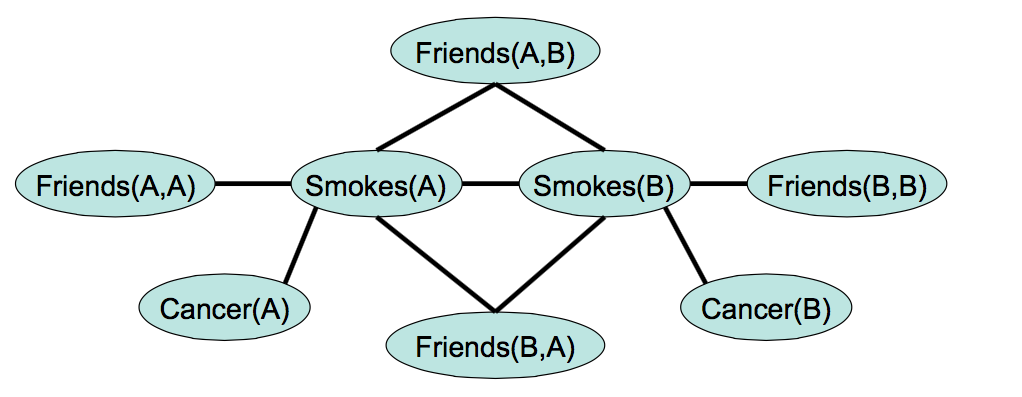
\includegraphics[scale=0.4]{mln}
  \caption{Beispiel}
\end{figure}

\mparagraph{Verbundswahrscheinlichkeit}
MLN ist eine Schablone für den Aufbau eines Markov Netzes. Die Wahrscheinlichkeit
einer Welt $X$ ist:
\begin{displaymath}
    P(X) = \frac{1}{Z}(\sum_{i}w_in_i(X))
\end{displaymath}
\begin{itemize}
    \item $w_i$: Gewicht der Formel $i$
    \item $n_i(X)$: Anzahl der wahren Belegung der Formeln $i$ in $X$.
\end{itemize}
Ein Beispiel für $n_i(X)$ könnte sein:
\begin{displaymath}
    n_i(X) = n_i(\text{smoking,cancer}) = \begin{cases}
                                                1, \text{ if} \neg\text{smoking}
                                                 \vee \text{cancer}\\
                                                0, \text{ otherwise}
                                        \end{cases}
\end{displaymath}

\mparagraph{Inferenz}
Mit MAP finden des wahrscheinlichsten Zustands der Welt (Variablen y,) gegeben Evidenzen
x (wahrscheinlichste Erklärung für y)

\begin{align}
    \argmax_y P(y | x) &= \frac{1}{Z} \exp(\sum_{i} w_i n_i(x, y))\\
         &= \sum_{i} w_i n_i(x, y)
     \end{align}
